\documentclass{article}
\pdfpagewidth=8.5in
\pdfpageheight=11in
\usepackage{ijcai21}
\usepackage{times}
\usepackage{soul}
\usepackage{url}
\usepackage[hidelinks]{hyperref}
\usepackage[utf8]{inputenc}
\usepackage[small]{caption}
\usepackage{graphicx}
\usepackage{amsmath}
\usepackage{amsthm}
\usepackage{booktabs}
\usepackage{algorithm}
\usepackage{algorithmic}
\urlstyle{same}

\usepackage{cleveref}
\crefname{figure}{figure}{figures}
\Crefname{figure}{Figure}{Figures}

\usepackage{tikz}
\usetikzlibrary{shapes}

\usepackage{showframe}

\newtheorem{proposition}{Proposition}
\newtheorem{corollary}{Corollary}

\newcommand{\citet}[1]{\citeauthor{#1} \shortcite{#1}}

\usepackage{complexity}

\pdfinfo{
/TemplateVersion (IJCAI.2021.0)
}

\title{Solving Graph Homomorphism and Subgraph Isomorphism Problems Faster Through Clique Neighbourhood Constraints}

\author{
Ciaran McCreesh$^1$
\and
Sonja Kraiczy$^2$
\affiliations
$^1$University of Glasgow\\
$^2$University of Oxford\\
\emails
ciaran.mccreesh@glasgow.ac.uk
}

\newcommand{\neighbourhood}{\operatorname{N}}
\newcommand{\vertexset}{\operatorname{V}}
\newcommand{\degree}{\operatorname{deg}}
\newcommand{\nds}{\operatorname{S}}

\begin{document}

\maketitle

\begin{abstract}
    Graph homomorphism problems involve finding adjacency-preserving mappings between two graphs.
    Many of these problems are theoretically hard, but can be solved quite efficiently in practice
    through constraint programming techniques.  This paper adapts techniques from the
    state-of-the-art in subgraph isomorphism solving to broader graph homomorphism problems, and
    introduces a new form of filtering based upon clique-finding. We evaluate these techniques
    empirically, and show they are effective in practice for the locally injective graph
    homomorphism and subgraph isomorphism problems, as well as giving the first practical constraint
    programming approach to finding general graph homomorphisms.
\end{abstract}

\section{Introduction}

A \emph{graph homomorphism} is a function between two graphs that maps adjacent vertices to adjacent
vertices. An injective graph homomorphism is more commonly known as a \emph{subgraph isomorphism}, a
\emph{locally injective homomorphism} is one which is injective when restricted to any individual
vertex and its neighbourhood \cite{DBLP:journals/csr/FialaK08}, and a homomorphism which is
surjective on edges is known as an \emph{epimorphism} \cite{DBLP:journals/dam/GayFMSS14}. Finding
any of these kinds of homomorphism between two given graphs is \NP-complete.  The subgraph
isomorphism problem arises in many practical applications, including ??, and as such there has been
a lot of research into finding algorithms which perform well empirically. Most approaches are based
either upon very fast but simple backtracking algorithms,
\cite{DBLP:journals/pami/CordellaFSV04,DBLP:journals/bmcbi/BonniciGPSF13,DBLP:conf/gbrpr/CarlettiFSV17}
which often but not always perform well on very easy instances, or upon constraint programming
algorithms
\cite{DBLP:journals/constraints/ZampelliDS10,DBLP:journals/ai/Solnon10,DBLP:conf/cp/AudemardLMGP14,DBLP:conf/cp/McCreeshP15,DBLP:conf/cpaior/ArchibaldDHMP019},
which have higher startup costs but that perform vastly better on harder instances and much more
consistently on easy instances \cite{DBLP:journals/jair/McCreeshPST18,DBLP:conf/gbrpr/Solnon19}. The
current state of the art is the Glasgow Subgraph Solver \cite{DBLP:conf/gg/McCreeshP020}, which is a
dedicated constraint programming solver for subgraph-finding problems. Much of its performance comes
from inference strategies based upon degrees and neighbourhood degree sequences
\cite{DBLP:journals/constraints/ZampelliDS10}, counting paths between vertices
\cite{DBLP:conf/cp/AudemardLMGP14,DBLP:conf/cp/McCreeshP15}, and cardinality reasoning
\cite{DBLP:journals/ai/Solnon10}, which can be used to eliminate many infeasible candidate
assignments without search.

One might hope that this inference would also be helpful for other graph homomorphism problem
variants. Indeed, this paper proves that many, but not all, of these strategies are also valid in
the locally injective case, and that simple distance filtering is valid for all homomorphisms.
However, we also show that \emph{none} of the other strategies are valid for finding homomorphisms
where there is no injectivity requirement. Finally, we introduce a new filtering technique that is
based upon finding a maximum clique in the neighbourhood of each domain vertex, and prove that this
technique is valid even in the general case. Although this new filtering technique involves solving
many additional \NP-complete problems as a preprocessing step, we demonstrate that it is effective
in practice, particularly for the non-injective problem where filtering allows a constraint
programming algorithm to solve instances over eight hundred times faster in aggregate, over a
collection of over fourteen thousand standard benchmark instances. This shows, for the first time,
that modern constraint programming techniques can be practical for less constrained graph
homomorphism finding problems; previous algorithmic approaches have focused instead upon worst-case
computational bounds
\cite{DBLP:journals/csr/FialaK08,DBLP:journals/ipl/Rzazewski14,DBLP:journals/tcs/ChaplickFHPT15},
whose practical utility has yet to be demonstrated. The empirical effectiveness of our results is
especially important because many current applications use subgraph isomorphism solvers only because
they perform well using off the shelf solvers, rather than because they exactly match ideal domain
requirements ??cite.

\section{Background and Theory}

We begin by introducing notation and terminology, and by giving the theoretical results which
support our implementation.

\paragraph{Graphs.} Let $G$ and $H$ be graphs. Let $v \in \vertexset(G)$ be a vertex of $G$. The
\emph{(open) neighbourhood} of $v$, written $\neighbourhood_G(v)$, is the set of vertices adjacent
to $v$ not including $v$ itself, whilst the closed neighbourhood of $v$, written
$\neighbourhood_G[v]$, is the neighbourhood of $v$ plus $v$. The \emph{degree} of a vertex, $\degree_G(v)$,
is the cardinality of its open neighbourhood. The \emph{neighbourhood degree sequence} of a vertex
is the sequence consisting of the degrees of its neighbours, in descending order. Given a vertex set
$S \subseteq \vertexset(G)$, the subgraph \emph{induced by} $S$, written $G[S]$, is the subgraph of
$G$ with only the vertices in $S$ together with all the edges between them. A \emph{clique} is a
subgraph where every vertex is adjacent to every other in the subgraph.

\paragraph{Homomorphisms.} A \emph{homomorphism} from $G$ to $H$ is a function mapping vertices of
$G$ to vertices of $H$, such that adjacent vertices in $G$ are mapped to adjacent vertices in $H$. A
homomorphism $h$ is \emph{locally injective} if for every vertex $w$, the restriction of $h$ to
$G[N_G[w]]$ is injective; if $h$ is injective globally we call it a \emph{(non-induced) subgraph
isomorphism}.

\paragraph{Loops.} A vertex which is adjacent to itself is called a \emph{loop}. By a careful reading
of the definition, any homomorphism must map loops onto loops---and indeed, the Glasgow Subgraph
Solver and this paper take this approach (although some other algorithm implementations do not). It
therefore follows that for the homomorphism \emph{decision} problem where there are no injectivity
constraints, any problem instance which has a loop in the codomain graph is trivially satisfiable,
although the \emph{counting} problem remains \#\P-hard \cite{DBLP:journals/rsa/DyerG00}.

\paragraph{Constraint programming.} A \emph{constraint satisfaction problem} is defined in terms of
a set of \emph{variables}, each of which has a \emph{domain} of possible \emph{values}, together
with a set of constraints; the goal is to give each variable a value from its domain, whilst
satisfying all of the constraints. Homomorphism problems have a natural representation as a
constraint satisfaction problem: we have a variable for each vertex in the domain graph, whose
values range over the codomain graph, and a set of constraints saying that adjacent vertices must be
mapped to adjacent vertices. For the injective variants, one or more \emph{all-different}
constraints are also present. A typical constraint programming approach to solving such a problem is
to combine inference through constraint propagation with an intelligent backtracking search.

\paragraph{Degree-based invariants.} Constraint programming techniques for finding
homomorphisms can be made much more effective by exploiting certain invariants. It is
straightforward to verify the following.

\begin{proposition}[neighbourhood degree sequences are preserved]\label{proposition:degreends}
    Suppose  $i$ is a locally injective homomorphism from a $G$ to  $H$. Let
    $v$ be any vertex. Then:
    \begin{enumerate}
        \item $i$ cannot map $v$ to a vertex of lower degree, $\degree_G(v) \le \degree_H(i(v))$.
        \item Furthermore, $v$ cannot be mapped to any vertex whose neighbourhood degree sequence is
            not pointwise greater than or equal to its own.
    \end{enumerate}
\end{proposition}
Since subgraph isomorphisms are in particular locally injective, these invariants also hold for
subgraph isomorphisms \cite{DBLP:journals/constraints/ZampelliDS10}; indeed, every recent constraint
programming approach for subgraph isomorphism finding make use of degrees and neighbourhood degree
sequences. The simplest way for a constraint programming algorithm to use these results is as unary
constraints, which are propagated when domains are initialised, before search begins. For each
domain representing a domain vertex, any value representing a codomain vertex whose degree or
neighbourhood degree sequence is too low may immediately be rejected.

\begin{figure}
    \hfill\,\begin{minipage}{3cm}
    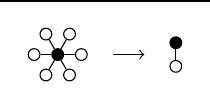
\begin{tikzpicture}
        \node [draw, fill, circle, inner sep=1.5pt] (A1) at (0, 0) {};
        \node [draw, circle, inner sep=1.5pt] (A2) at (0:0.3) {};
        \node [draw, circle, inner sep=1.5pt] (A3) at (60:0.3) {};
        \node [draw, circle, inner sep=1.5pt] (A4) at (120:0.3) {};
        \node [draw, circle, inner sep=1.5pt] (A5) at (180:0.3) {};
        \node [draw, circle, inner sep=1.5pt] (A6) at (240:0.3) {};
        \node [draw, circle, inner sep=1.5pt] (A7) at (300:0.3) {};

        \draw (A1) -- (A2);
        \draw (A1) -- (A3);
        \draw (A1) -- (A4);
        \draw (A1) -- (A5);
        \draw (A1) -- (A6);
        \draw (A1) -- (A7);

        \draw [->] (0.7, 0) -- (1.1, 0);

        \draw (1.5, 0) node [draw, fill, circle, inner sep=1.5pt] (B1) at ++ (90:0.15) {};
        \draw (1.5, 0) node [draw, circle, inner sep=1.5pt] (B2) at ++ (270:0.15) {};
        \draw (B1) -- (B2);
    \end{tikzpicture}\end{minipage}\hfill\begin{minipage}{3cm}
    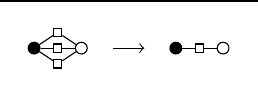
\begin{tikzpicture}
        \node [draw, fill, circle, inner sep=1.5pt] (A1) at (0, 0) {};
        \node [draw, inner sep=1.5pt] (A2) at (0.3, 0) {};
        \node [draw, inner sep=1.5pt] (A3) at (0.3, -0.2) {};
        \node [draw, inner sep=1.5pt] (A4) at (0.3, 0.2) {};
        \node [draw, circle, inner sep=1.5pt] (A5) at (0.6, 0) {};

        \draw (A1) -- (A2);
        \draw (A1) -- (A3);
        \draw (A1) -- (A4);
        \draw (A2) -- (A5);
        \draw (A3) -- (A5);
        \draw (A4) -- (A5);

        \draw [->] (1.0, 0) -- (1.4, 0);

        \node [draw, fill, circle, inner sep=1.5pt] (B1) at (1.8, 0) {};
        \node [draw, inner sep=1.5pt] (B2) at (2.1, 0) {};
        \node [draw, circle, inner sep=1.5pt] (B5) at (2.4, 0) {};

        \draw (B1) -- (B2);
        \draw (B2) -- (B5);
    \end{tikzpicture}\end{minipage}\hfill\,

    \bigskip

    \,\hfill\begin{minipage}{3cm}
    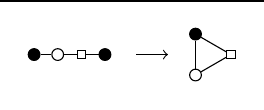
\begin{tikzpicture}
        \node [draw, fill, circle, inner sep=1.5pt] (A1) at (0, 0) {};
        \node [draw, circle, inner sep=1.5pt] (A2) at (0.3, 0) {};
        \node [draw, inner sep=1.5pt] (A3) at (0.6, 0) {};
        \node [draw, fill, circle, inner sep=1.5pt] (A4) at (0.9, 0) {};

        \draw (A1) -- (A2);
        \draw (A2) -- (A3);
        \draw (A3) -- (A4);

        \draw [->] (1.3, 0) -- (1.7, 0);

        \draw (2.2, 0) node [draw, fill, circle, inner sep=1.5pt] (B1) at ++ (120:0.3) {};
        \draw (2.2, 0) node [draw, circle, inner sep=1.5pt] (B2) at ++ (240:0.3) {};
        \draw (2.2, 0) node [draw, inner sep=1.5pt] (B3) at ++ (0:0.3) {};

        \draw (B1) -- (B2);
        \draw (B2) -- (B3);
        \draw (B3) -- (B1);
    \end{tikzpicture}\end{minipage}\hfill\begin{minipage}{3cm}
        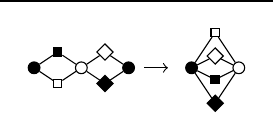
\begin{tikzpicture}
        \node [draw, fill, circle, inner sep=1.5pt] (A1) at (0, 0) {};
        \node [draw, inner sep=1.5pt] (A2) at (0.3, -0.2) {};
        \node [draw, fill, inner sep=1.5pt] (A3) at (0.3, 0.2) {};
        \node [draw, circle, inner sep=1.5pt] (A4) at (0.6, 0) {};
        \node [draw, diamond, fill, inner sep=1.5pt] (A5) at (0.9, -0.2) {};
        \node [draw, diamond, inner sep=1.5pt] (A6) at (0.9, 0.2) {};
        \node [draw, fill, circle, inner sep=1.5pt] (A7) at (1.2, 0) {};

        \draw (A1) -- (A2);
        \draw (A1) -- (A3);
        \draw (A2) -- (A4);
        \draw (A3) -- (A4);
        \draw (A4) -- (A5);
        \draw (A4) -- (A6);
        \draw (A5) -- (A7);
        \draw (A6) -- (A7);

        \draw [->] (1.4, 0) -- (1.7, 0);

        \node [draw, fill, circle, inner sep=1.5pt] (B1) at (2, 0) {};
        \node [draw, fill, inner sep=1.5pt] (B2) at (2.3, -0.15) {};
        \node [draw, diamond, inner sep=1.5pt] (B3) at (2.3, 0.15) {};
        \node [draw, diamond, fill, inner sep=1.5pt] (B4) at (2.3, -0.45) {};
        \node [draw, inner sep=1.5pt] (B5) at (2.3, 0.45) {};
        \node [draw, circle, inner sep=1.5pt] (B6) at (2.6, 0) {};

        \draw (B1) -- (B2);
        \draw (B1) -- (B3);
        \draw (B1) -- (B4);
        \draw (B1) -- (B5);
        \draw (B6) -- (B2);
        \draw (B6) -- (B3);
        \draw (B6) -- (B4);
        \draw (B6) -- (B5);
    \end{tikzpicture}\end{minipage}\hfill\,

    \caption{Counter-examples for various properties which are not invariants. The different shapes
        for vertices show a mapping, with vertices being mapped to vertices of the same shape. The
        top left example shows that degree is not preserved in a homomorphism; the top right that path
        counts are not preserved in a homomorphism; the bottom left that path counts of length three
        are not preserved in a locally injective homomorphism; and the bottom right that a locally
        injective homomorphism $i$ can give rise to a homomorphism $i^{2,2}$ which is not locally
        injective.} \label{figure:counterexamples}
\end{figure}

However, these invariants do \emph{not} hold for homomorphisms in general. As a simple
counter-example, a homomorphism may map a star graph onto a single edge, as in
\cref{figure:counterexamples} (top left).

\paragraph{Path-based invariants.} Constraint programming solvers can also exploit
invariants that are based upon paths. This is done by automatically adding \emph{implied}
constraints to the problem that are implied by the original model, but that will give stronger
propagation power.

\begin{proposition}[paths are preserved by subgraph isomorphisms]\label{proposition:distances}For
    the problem of finding a subgraph isomorphism $i$ from a graph $G$ to a graph $H$, the following
    constraints are implied for any pair of vertices $v, w \in \vertexset(G)$:
    \begin{enumerate}
        \item The distance between $v$ and $w$ is at least the distance between $i(v)$ and $i(w)$
            \cite{DBLP:conf/cp/AudemardLMGP14}.
        \item If there are at least $k$ simple
            paths of length exactly $\ell$ between $v$ and $w$, then there must be at least $k$
            simple paths of length exactly $\ell$ between $i(v)$ and $i(w)$
            \cite{DBLP:conf/cp/McCreeshP15}.
    \end{enumerate}
\end{proposition}

It is easy to verify that the first of these two properties is valid for \emph{any} homomorphism.
The second property does not hold for homomorphisms in general: for example, a pair of vertices
connected by three paths of length two may be mapped onto a pair of vertices connected by a single
path of length two (see \cref{figure:counterexamples}, top right). Local injectivity is trickier.
The second property does not hold in full generality, because, for example, a path of length three
may be mapped onto a triangle whilst respecting local injectivity (\cref{figure:counterexamples},
bottom left).  However, we observe that a weaker result holds:

\begin{proposition}[paths of length two are preserved by locally injective
    homomorphisms]\label{proposition:paths}For the problem of finding a locally injective graph
    homomorphism $i$ from a graph $G$ to a graph $H$, for any pair of vertices $v, w \in
    \vertexset(G)$, if there are at least $k$ simple paths of length exactly two between $v$ and
    $w$, then there must be at least $k$ simple paths of length exactly two between $i(v)$ and
    $i(w)$.
\end{proposition}

\begin{proof}Let $\{ x_1, \ldots, x_n \}$ be the intermediate vertices on the paths of length two
between $v$ and $w$. Observe that each $x_j$ is in the neighbourhood of $v$, and so must be mapped
    to different vertices. Thus each sequence $(i(v), i(x_j), i(w))$ gives a distinct simple path of
length two between $i(v)$ and $i(w)$ as required.\end{proof}

Rather than using distance properties directly, \citet{DBLP:conf/cp/McCreeshP15} introduced
the notion of \emph{supplemental} graphs, with the idea that a constraint programming algorithm can
search for a mapping which is simultaneously a subgraph isomorphism between several different pairs
of graphs. Let $G^d$ be the graph with the same set of vertices as $G$, but an edge between vertices
$v$ and $w$ if the distance between $v$ and $w$ in $G$ is at most $d$.  Similarly, let $G^{n,\ell}$
be the graph with the same set of vertices as $G$, but an edge between vertices $v$ and $w$ if there
are at least $n$ simple paths of length exactly $\ell$ between $v$ and $w$ in $G$. Following on from
\cref{proposition:distances,proposition:paths}, we generalise the result of
\citeauthor{DBLP:conf/cp/McCreeshP15} as follows.

\begin{corollary}Any homomorphism $i$ from $G$ to $H$ gives a homomorphism $i^d$ from $G^d$ to $H^d$
    defined by $i^d(v) = i(v)$, for all $d$. Furthermore, if $i$ is locally injective, then for all
    $n$, there is a homomorphism $i^{n,2}$ from $G^{n,2}$ to
    $H^{n,2}$ defined by $i^{n,2}(v) = i(v)$.\label{corollary:lishapes}
\end{corollary}

Note carefully that $i^{n,2}$ is \emph{not} necessarily locally injective, even if $i$ is; we
illustrate a counter-example in \cref{figure:counterexamples} (bottom right). This is in contrast to
subgraph isomorphism, where $i^{n,\ell}$ is a subgraph isomorphism for all $\ell$
\cite{DBLP:conf/cp/McCreeshP15}.

\paragraph{Cliques and homomorphisms.} Finally, we come to the main result of this paper. Observe
that until now, we have not seen any unary constraints which are valid for the general homomorphism
problem. All existing constraint programming approaches for the subgraph isomorphism problem begin
by branching on the variable which has the smallest domain---typically this will be a domain for a
domain vertex of high degree, or which has many high degree neighbours. Furthermore, once one such
guessed assignment has been made, adjacency propagation means many other domains will be
substantially reduced in size, making subsequent branching choices simpler.  However, for
homomorphism problems, if we cannot find any implied unary constraints then every domain will
initially be of the same size, which will make it much harder for a solver to know where to start.
This motivates the following observation.

\begin{proposition}[Cliques are preserved]\label{proposition:clique}
    Let $i$ be a homomorphism from $G$ to $H$ where $H$ does
    not contain any loops. Let $S\subset V$ be such that $G[S]$ is a $k$-vertex clique. Then
    $H[i(S)]$ is also a $k$-vertex clique.
\end{proposition}

\begin{proof}
    Let $j$ and $k$ be two distinct vertices of the clique in $G$. By definition of a homomorphism,
    $i(j)$ and $i(k)$ must be adjacent. And, because $H$ does not contain loops, $i(j)$ cannot equal
    $i(k)$.
\end{proof}

\begin{corollary}\Cref{proposition:clique} holds for locally injective graph homomorphisms and for
    subgraph isomorphisms even if loops are present in the second graph.
\end{corollary}

We will discuss how this is useful in practice in the following section.

\section{Design and Implementation}

Having determined which commonly-used subgraph isomorphism invariants do and do not hold for other
forms of homomorphism, and having discovered a new clique-based invariant, we will now look at how
these invariants may be used in practice. Our starting point is the Glasgow Subgraph Solver
\cite{DBLP:conf/gg/McCreeshP020}, due to it being the current single strongest solver for the
subgraph isomorphism problem. Adapting the solver to handle locally injective and general
homomorphism problems required the following straightforward changes.

\paragraph{Injectivity constraints.} For subgraph isomorphism, injectivity is handled by a
combination of binary constraints and a specialised bit-parallel all-different propagator
\cite{DBLP:conf/cp/McCreeshP15}. This was disabled entirely for homomorphism problems, and for local
injectivity only binary constraints were used.

\paragraph{Path-based filtering.} For subgraph isomorphism, the Glasgow Subgraph Solver
searches for a mapping which is simultaneously a subgraph isomorphisms between $(G, H)$ and each
$(G^{n,2}, G^{n,2})$ for each $n$ from $1$ to $4$, and optionally also between $(G^3, H^3)$.

\paragraph{Degree-based filtering.} This was disabled for homomorphisms and left enabled for locally
injective homomorphisms, as per \cref{proposition:degreends}. For subgraph isomorphism, the Glasgow
Subgraph Solver uses degree and neighbourhood degree sequences not just on the original graphs, but
also on each $(G^{n,\ell}, H^{n,\ell})$ graph pair. This is \emph{not} possible for locally
injective homomorphisms, due to the counter-example following \ref{corollary:lishapes}.

\paragraph{Search order heuristics.} The solver's default search order heuristics are based upon
three principles: that it is good to branch on variables with few remaining values in a domain, that
it is good to branch on variables corresponding to high-degree vertices, and that it is good to try
mapping to vertices of high degree
\cite{DBLP:journals/jair/McCreeshPST18,DBLP:conf/cpaior/ArchibaldDHMP019}. These principles do not
appear to be specific to subgraph isomorphism, and so we do not alter the search order heuristics.

\paragraph{Loops.} For the homomorphism decision problem, we modified the solver so that if the
codomain graph contains a loop, we immediately return a satisfying assignment mapping every vertex
to the loop.

\subsection{Clique Filtering}

Implementing clique constraints required substantially more work. The Glasgow Subgraph Solver
contains a maximum clique implementation, which is based upon a variation of
\citet{DBLP:conf/walcom/TomitaSHTW10}'s MCS algorithm which
\citet{DBLP:journals/algorithms/Prosser12} calls ``MCSa1'', with bit-parallelism and an altered
branching scheme for faster optimality proofs \cite{DBLP:conf/cp/McCreeshP14}. The implementation
also makes use of a shortcut due to \citet{DBLP:journals/jco/BatsynGMP14}, which allows certain
cliques to be detected without branching---this turns out to be particularly useful in this setting,
making many of the clique instances generated solvable using only a single greedy colouring step.
Initially we used this solver to perform domain filtering as a preprocessing step. Preliminary
experiments showed that a na{\"\i}ve approach, which simply calculates the maximum clique size for
the neighbourhood of each domain vertex and each codomain vertex, would add as much as three minutes
of preprocessing time to some problem instances which could otherwise be solved in a few seconds. We
therefore use a more intelligent approach, which we now describe.

Assuming a problem instance is not detected as obviously unsatisfiable, we calculate the maximum
clique size for the neighbourhood of every domain vertex in turn. However, having found the maximum
clique with $k$ vertices in the neighbourhood of a vertex $p$, we remember for every other vertex in
the maximum clique that its neighbourhood maximum clique size is at least $k$. This can be used to
accelerate subsequent clique solver calls, by starting the branch and bound algorithm with an
initial incumbent size of $k$ rather than zero.

We then move on to the codomain vertices, using a similar caching routine. Rather than calculating a
clique size for every single codomain vertex, we only calculate a value for codomain vertices which are
present in at least one variable's domain, after other unary constraints have been applied.
(Depending upon the problem variant, implied constraints like degree and neighbourhood degree
sequence can eliminate some codomain vertices from the domains of all domain variables.)
Additionally, we do not require the maximum clique solver to run to completion and guarantee that it
has found a maximum clique. Instead, we allow it to stop as soon as it has found a clique with as
many vertices as the largest domain clique. This is useful in practice because it may be very hard
to decide whether a particular codomain vertex has neighbourhood clique size of, say, 15 or 16, but if
the largest domain vertex has a neighbourhood clique size of only 5 then this is irrelevant.

?? Why this works. Clique finding is much easier, colour bounds, etc. Small graphs. ?? See in
section blah that it's really fast.

\subsection{Proof Logging}

Given the complexity of implementations of modern solvers, a critical question is how we can be sure
that they are producing correct answers. The Glasgow Subgraph Solver's subgraph isomorphism and
clique algorithms are both \emph{certifying} \cite{DBLP:journals/csr/McConnellMNS11}: that is, they
can output a mathematical proof that they have reached a correct answer by sound reasoning, and this
proof log can be verified by the VeriPB proof checking tool
\cite{DBLP:conf/cp/GochtMMNPT20,DBLP:conf/ijcai/GochtMN20}. Certification involves two stages:
firstly, the solver translates its inputs into a pseudo-Boolean model (this part is not verified),
and secondly (for unsatisfiable instances), the solver provides a proof using cutting planes rules
and reverse unit propagation steps that the pseudo-Boolean model is unsatisfiable.

Implementing proof-logging for the changes not involving clique-finding was routing---although proof
logging did catch an implementation bug where we were incorrectly applying degree-based filtering on
the $G^{2,n}$ graphs for locally injective homomorphisms, in violation of the counter-example to
\cref{corollary:lishapes}. For clique-based filtering, more work was required. We briefly
outline the steps taken to implement proof logging for the fact that a vertex $p$ in the domain
graph which is present in a $k$-vertex clique cannot be mapped to a vertex $t$ in the codomain graph
which is not present in a $k$-vertex clique.

?? Many technicalities.

We have an $x_{p{,}t}$ saying that $p$ gets mapped to $t$. For a regular clique problem, we would have
binary constraints $\overline{x}_i + \overline{x}_j \ge 1$ for each non-adjacent vertex $i$ and
$j$. We wish to derive something similar for the non-adjacent vertices in the neighbourhood of $t$.
However, our constraints are conditional upon $p$ being mapped to $t$, and so instead we start our
proof step by deriving three sets of conditional\footnote{For the subgraph isomorphism case, these
constraints need not be conditional.} pseudo-adjacency constraints:
\begin{itemize}
    \item $\overline{x}_{p{,}t} + \overline{x}_{q{,}u} + \overline{x}_{r{,}v} \ge 1$
    \item $\overline{x}_{p{,}t} + \overline{x}_{q{,}u} + \overline{x}_{r{,}u} \ge 1$
    \item $\overline{x}_{q{,}u} + \overline{x}_{q{,}v} \ge 1$
\end{itemize}
Each of these constraints follows by reverse unit propagation from the original model, and so
requires no further justification in a proof log. We also need an objective constraint. From the
definition of the homomorphism problem, we have existing adjacency constraints $\overline{x}_{p{,}t}
+ \sum_{u \in \neighbourhood(t)} x_{q{,}u} \ge 1$, and we may sum these constraints for each of the
$k - 1$ vertices in the $k$-clique that includes $p$ to express that a suitable $k$-clique must
exist in the codomain graph.

We have now established something that is sufficiently similar to the maximum clique model used by
?? that the . Colour classes (used for bounds) are in correspondence with colour classes in this
adapted problem instance, which is similar to microstructure. Produce a proof that there is no
target clique. The condition appears in the trail, and rather than deriving a contradiction, gets
$\overline{x}_{p,t} \ge 1$.

This situation is not entirely ideal. The proofs produced this way are inherently dependent upon a
\emph{particular} choice of $p$ and $t$ vertices. When not proof logging, we need to solve a single
maximum clique problem for each vertex in the domain, and a restricted clique problem for each
vertex in the codomain. With proof logging, we must instead solve restricted clique problems for
each $(p, t)$ assignment that is to be filtered, which is potentially a linear factor blowup. This
feels morally excessive, since for any given $t$ (and for any clique in the codomain graph which is
reused) the proofs produced are effectively the same up to a substitution of variable names. We
would therefore be interested in seeing a proof system extension which would allow us to avoid this
duplication.

\section{Experiments}

\begin{figure*}[p]
    \,\hfill\begin{tabular}{c@{}c@{}c@{}}
    \includegraphics{gen-graph-cumulatives.pdf}
        &
    \includegraphics{gen-graph-cumulatives-differences.pdf}
        &
    \includegraphics{gen-graph-cumulatives-aggregate.pdf}
        \\[5mm]
    \includegraphics{gen-graph-cumulatives-hom.pdf}
        &
    \includegraphics{gen-graph-cumulatives-local.pdf}
        &
    \includegraphics{gen-graph-cumulatives-si.pdf}
    \end{tabular}\hfill\,

    \caption{On the top left, the cumulative number of instances solved over time for the three
    problem variants, with and without clique filtering, and with and without distance filtering for
    the homomorphism problem; for comparison, results for subgraph isomoprhism using the PathLAD,
    RI, and VF2 solvers are also shown. The remaining plots re-display this data, as follows. The
    three plots on the bottom row zoom in on the cumulative number of instances solved, for the
    homomorphism problem on the left, the locally injective homomorphism problem in the centre, and
    the subgraph isomorphism problem on the right. The top centre plot shows the additional number
    of instances solved at any given time when using the new forms of filtering for all problem
    variants, and the top right plot shows the aggregate speedups from each form of filtering.}
\end{figure*}
\begin{figure*}[p]
    \,\hfill\begin{tabular}{c@{\hspace{4mm}}c@{\hspace{4mm}}c@{\hspace{4mm}}c@{\hspace{4mm}}}
        \includegraphics{gen-graph-scatter-hom-c.pdf}
        &
        \includegraphics{gen-graph-scatter-hom-cd.pdf}
        &
        \includegraphics{gen-graph-scatter-local.pdf}
        &
        \includegraphics{gen-graph-scatter-si.pdf}
    \end{tabular}\hfill\,

    \caption{Looking at the effects of additional filtering on an instance by instance basis, for
    homomorphism with just clique filtering and with both clique and distance filtering, and for the
    other two variants with clique filtering. Each point represents one instance, the vertical axis
    is the runtime with filtering in ms, and the horizontal axis is the runtime without filtering in
    ms (and so points below the diagonal are speedups). Points on the outer axes are timeouts. The
    different point styles show the different families of instance from the benchmark set, and
    illustrate that in each the filtering is broadly useful rather than being specific to a single
    kind of application.}
\end{figure*}

We now evaluate this approach empirically on 

?? How good is it

?? Time on cliques

?? Whether cliques are hard

?? Loops

\section{Conclusion and Future Work}

?? Neighbourhood colourability? Cores?

?? Epimorphism

\section*{Acknowledgements}

This work was supported by the Engineering and Physical Sciences Research Council [grant number
EP/P026842/1].

\bibliographystyle{named}
\bibliography{paper}

\end{document}

% vim: set tw=100 spell spelllang=en : %
